
\documentclass[journal]{IEEEtran}
\usepackage{blindtext}
\usepackage{graphicx}
\usepackage[T2A]{fontenc}			% кодировка
\usepackage[utf8]{inputenc}	
\usepackage[english, russian]{babel}
\usepackage{subfigure}
\usepackage{wrapfig}
\usepackage{caption}
\usepackage[usenames]{color}
\usepackage{colortbl}
\usepackage{float}

\ifCLASSINFOpdf
\else
\fi
\usepackage[cmex10]{amsmath}

\usepackage[document]{ragged2e}


\begin{document}
\title{\small}
\markboth{ОТЧЕТ. Расчетные спектры Трехкристальной Рентгеновской Дифрактометрии (ТРД) – \today}
{TRTATATA \MakeLowercase{\textit{Аткнин Иван}}: ФНИЦ Кристаллография}


% \maketitle

%-----------------------1---------------------------

\textcolor{BrickRed}{\section{Интенсивность}}
В результате трехкратного отражения луча, выходящего из источника рентгеновского 
излучения, на выходе получаем двумерное распределение интенсивности (\ref{eqn: intensity}):

\begin{eqnarray}
\label{eqn: intensity}
	 I(\varepsilon,\omega, \theta, \lambda) =  \iint d\theta d\lambda g_\lambda(\lambda)  g_\theta(\theta) 
	 R_M\left(\theta-\frac{\lambda-\lambda_1}{\lambda_1}\tan\Theta_B \right) \cdot \nonumber \\  
	R_S\left(\omega+\theta-\frac{\lambda-\lambda_1}{\lambda_1}\tan\Theta_B\right) \cdot \nonumber \\  
	R_A\left(2\omega - \varepsilon+\theta-\frac{\lambda-\lambda_1}{\lambda_1}\tan\Theta_B\right),
\end{eqnarray}

где $\omega$ - угол поворота образца относительно угла Брегга ($\Theta - \theta_B$);
$\varepsilon$  - угол поворота анализатора относительно угла Брегга;  $g_\lambda(\lambda)$, $g_\theta(\theta)$ – функции спектрального и углового распределения падающего рентгеновского пучка; 

\hrulefill \\

\textcolor{BrickRed}{\section{Отклонение вектора дифракции}}
\begin{eqnarray}
\label{eqn: qx_qz}
	 q_x = k_0 (2\omega - \varepsilon) \cdot sin(\theta_B) \\
	 q_z = k_0 \varepsilon \cdot cos(\theta_B) 
\end{eqnarray}

\textcolor{BrickRed}{\section{Анализ пиков}}
\textcolor{BrickRed}{\subsection{Главный пик(ГП)}}
$$I_{max} = R_M(0) \cdot R_S(\omega) \cdot R_A(0)$$
$2\omega = \varepsilon$; 
$q_x = 0$.
\textcolor{BrickRed}{\subsection{Псевдо пик монохроматора(ППМ)}}
$$I_{max} = R_M(-\omega) \cdot R_S(0) \cdot R_A(0)$$
$\varepsilon = \omega$; 
$\frac{q_z}{q_x} = ctg(\theta_B)$.
\textcolor{BrickRed}{\subsection{Главный пик анализатора(ППА)}}
$$I_{max} = R_M(0) \cdot R_S(0) \cdot R_A(-\varepsilon)$$
$\omega = 0$; 
$\frac{q_z}{q_x} = -ctg(\theta_B)$.

\hrulefill \\

\textcolor{BrickRed}{\section{Эксперимент Ge-Si-Ge}}
Рентгеновский эксперимент выполнялся с использование кристаллов:


-образец Si(220), $\theta_B = 10.64^o$;

-монохроматор и анализатор Ge(220),  $\theta_B = 10.21^o$;

\begin{figure}[H]
\centering
\includegraphics[width=1\linewidth]{img/exp_linear.eps}
\caption{Карта распределения интенсивности рассеяния в окрестности узла обратной решетки 220 
в координата $\varepsilon$ и $\omega$. Логарифмический масштаб}
\label{ris:mapexper1}
\end{figure}


\begin{figure}[H]
\centering
\includegraphics[width=1\linewidth]{img/exp_qx_qz.eps}
\caption{Карта распределения интенсивности рассеяния в окрестности узла обратной решетки 220 
в координатах $q_x, q_z$. Логарифмический масштаб}
\label{ris:mapexper2}
\end{figure}


\hrulefill \\
\clearpage

\textcolor{BrickRed}{\section{Расчет Ge-Si-Ge}}

-образец Si(220), $\theta_B = 10.64^o$, $\chi_0 = \frac{(-31.745 + i0.1606)}{10^{7}}$, 
$\chi_h = \frac{(19.210 + i0.15497)}{10^{7}}$;

-монохроматор и анализатор Ge(220),  $\theta_B = 10.21^o$, $\chi_0 = \frac{(-64.169 + i3.6674 )}{10^{7}}$, 
$\chi_h = \frac{(46.505 + i3.5577)}{10^{7}}$;

\begin{figure}[H]
\centering
\includegraphics[width=1\linewidth]{img/theor_linear.eps}
\caption{Карта распределения интенсивности рассеяния в окрестности узла обратной решетки 220 
в координата $\varepsilon$ и $\omega$. Логарифмический масштаб}
\label{ris:maptheor1}
\end{figure}

\begin{figure}[H]
\centering
\includegraphics[width=1\linewidth]{img/theor_qx_qz.eps}
\caption{Карта распределения интенсивности рассеяния в окрестности узла обратной решетки 220 
в координата $q_x, q_z$. Логарифмический масштаб}
\label{ris:maptheor2}
\end{figure}

\textcolor{BrickRed}{\section{Расчет Si-Si-Si}}

-образец Si(220), $\theta_B = 10.64^o$, $\chi_0 = \frac{(-31.745 + i0.1606)}{10^{7}}$, 
$\chi_h = \frac{(19.210 + i0.15497)}{10^{7}}$;

\begin{figure}[H]
\centering
\includegraphics[width=1\linewidth]{img/si_si_si_linear.eps}
\caption{Карта распределения интенсивности рассеяния в окрестности узла обратной решетки 220 
в координата $\varepsilon$ и $\omega$. Логарифмический масштаб}
\label{ris:maptheor1}
\end{figure}

\begin{figure}[H]
\centering
\includegraphics[width=1\linewidth]{img/si_si_si_qx_qz.eps}
\caption{Карта распределения интенсивности рассеяния в окрестности узла обратной решетки 220 
в координата $q_x, q_z$. Логарифмический масштаб}
\label{ris:maptheor2}
\end{figure}
% \hrulefill \\
% \textcolor{BrickRed}{\section{Травление}}
% В качестве травителя взят раствор HNO3 – H2O в концентрации 1 – 1 соответственно. 

% Температура: $50^oC$

% Общее время травления: 30 мин.


% \hrulefill \\
% \textcolor{BrickRed}{\section{Эскизы}}
% В колличествое 6 штук.
% \begin{figure}[h]
% \centering
% \includegraphics[width=1\linewidth]{img/eskiz.eps}
% \caption{Эскиз образцов}
% \label{ris:eskiz}
% \end{figure}

% \hrulefill \\
% %-----------------------2---------------------------
% \textcolor{BrickRed}{\section{Напыление}}
% Нанесение электродов осуществлялось в НИЦ КИ на
% установке магнетронного напыления. Была сделана подложка диаметром 
% 151 мм, к которой особым образом крепились образцы (Рис.~\ref{ris:maska}):
% \begin{figure}[h]
% \centering
% \includegraphics[width=1\linewidth]{img/mask.eps}
% \caption{А)Подложка  В)Маска для напыления
% электродов}
% \label{ris:maska}
% \end{figure}

% \begin{figure}[h]
% \centering
% \includegraphics[width=1\linewidth]{img/napylen.eps}
% \caption{Результат напыления и КДО}
% \end{figure}
% \hrulefill \\



% \textcolor{BrickRed}{\section{Выбор метода}}
% Чтобы продемонстрировать пьзоэффект в кристалле, давайте встанем в произвольную точку 
% на кривой дифракционного отражения, другими словами выведем интенсивность детектора 
% из максимума отражения в точку на склоне кривой (Рис.~\ref{ris:kdopiez}).

% \begin{figure}[h]
% \centering
% 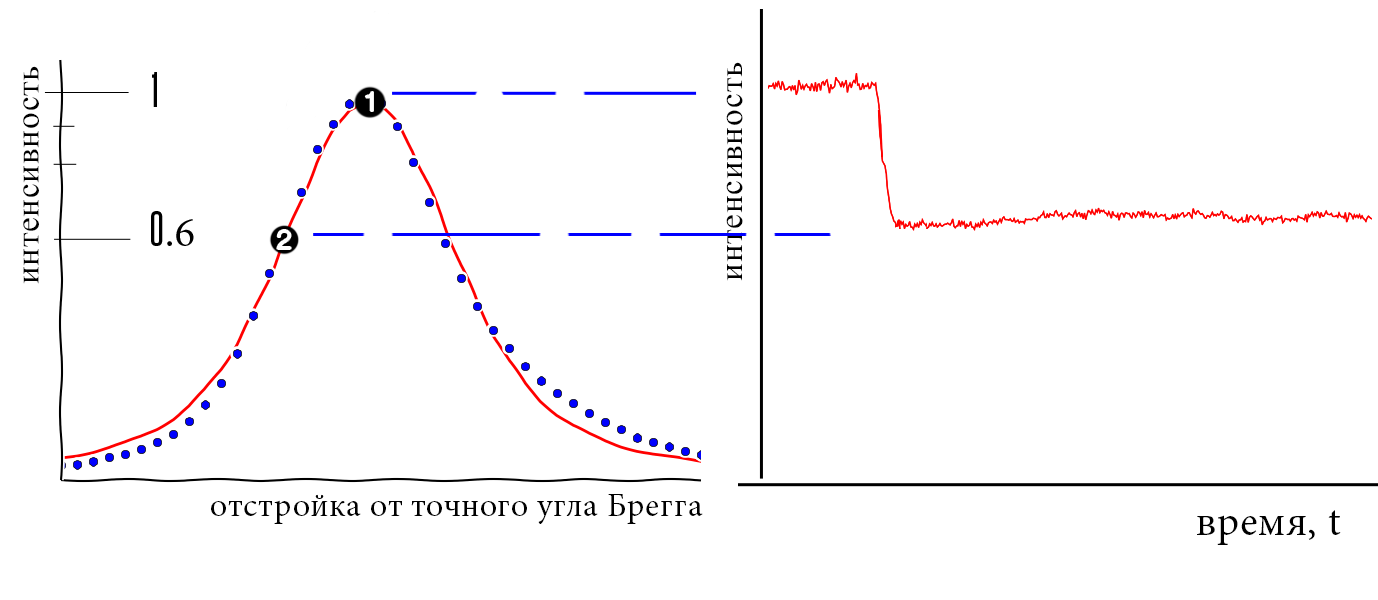
\includegraphics[width=1\linewidth]{img/kdopiez.eps}
% \caption{Выбор точки на КДО(справа), интенсивность сигнала детектора}
% \label{ris:kdopiez}
% \end{figure}

% \par
% Теперь включим электрическое поле поочередно в разных направлениях (Рис.~\ref{ris:princip}B). 
% \par
% Наблюдаем смещение кривой (Рис.~\ref{ris:princip}C), т.е. прямое изменение интенсивности на детекторе (Рис.~\ref{ris:princip}A).

% \begin{figure}[h]
% \centering
% 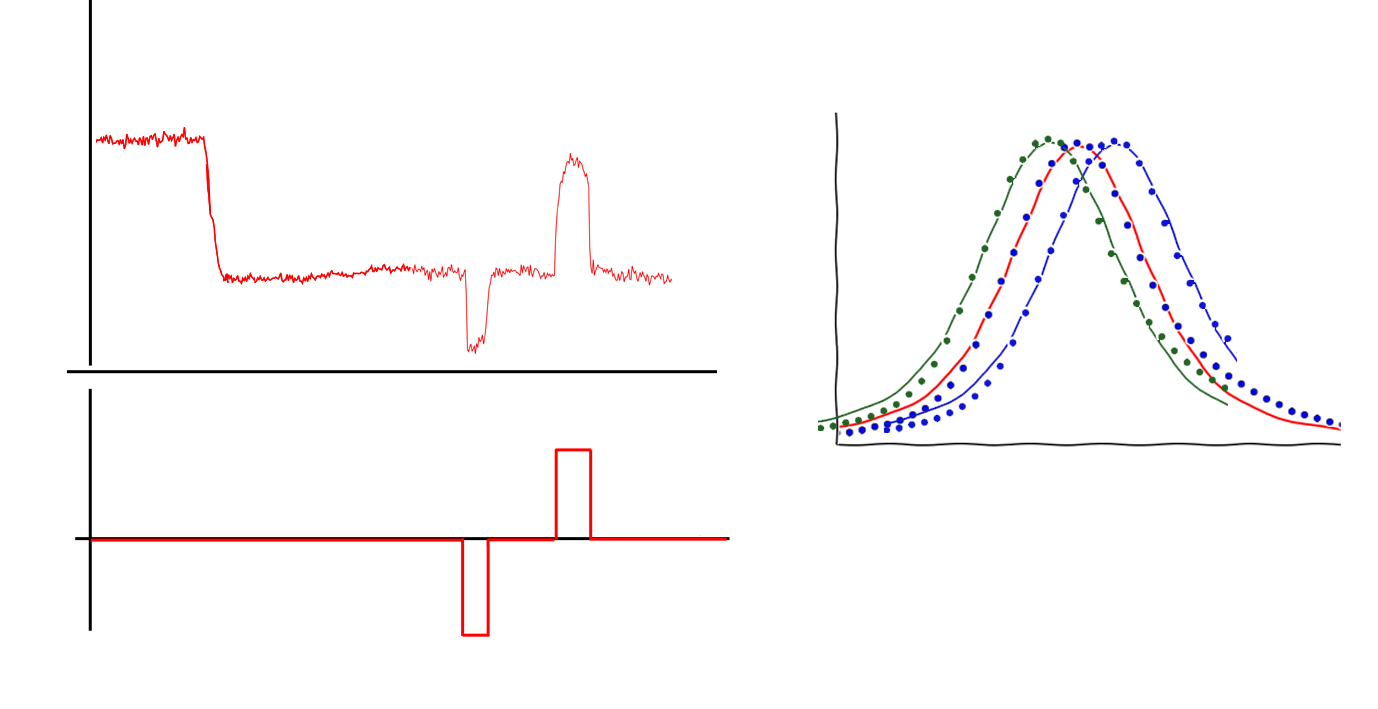
\includegraphics[width=1\linewidth]{img/princip.eps}
% \caption{A) Интенсивность детектора; В) Разность потенциалов на 
% поверхности кристалла; С) Положение КДО}
% \label{ris:princip}
% \end{figure}

% Таким образом представлется возможным отследить перемещение выбранного количества точек на КДО в момент подачи поля на кристал. Это позволит нам оценить искомый модуль (d33) обратного пьезоэффекта. Исключить ``паразитные'' вклады в смещение кривой и сократить ошибку. Так например кристал LBO имеет коэффициент теплового расширения в 7 раз превышающий величину для кристаллов кварца и кремния (2:14), ниже будет показано влияние температуры на отражение. К тому же, наблюдается уширение кривой, а так же смещения в связи с неизвестными нам эффектами, но к нашему везению, время действия пьезоэффекта на порядок меньше времени тех процессов которые были перечислены (покажем это ниже). Подробный список наблюдений, оказывающих ряд трудностей для измерения - приведен в приложении А. Избежать дополнительных эффектов удалось, проводя разовые эксперименты, с промежуточными перерывами в 1 час.


% \hrulefill \\


% \textcolor{BrickRed}{\section{Эксперимент}}
% Колличество измерений проведенного для оценки модуля $d_{33}$ - 1000. 


% \textcolor{BrickRed}{\subsection{1200 В}}
% {
% Величина такого смещения составляет: $\delta\theta = 2.60 \pm 0.01$ уг. сек (Рис~\ref{ris:1200_kdo}). 
% \begin{figure}[h]
% \centering
% \includegraphics[width=1\linewidth]{img/1200_kdo.eps}
% \caption{На рисунке представлено смещение КДО в результате обратного пьезоэффекта. Красным - в отсутствии поля, черным - в присутствии поля, 1200В}
% \label{ris:1200_kdo}
% \end{figure}
% }


% \textcolor{BrickRed}{\subsection{-1200 В}}
% {
% Измерения проводились независимым образом, с промежутком в 1 час
% $\delta\theta = -3.62 \pm 0.36$ уг. сек.(Рис~\ref{ris:-1200_kdo});

% $d_{33} = 34\cdot10^{-12}$
% \begin{figure}[h]
% \centering
% \includegraphics[width=1\linewidth]{img/-1200_kdo.eps}
% \caption{На рисунке представлено смещение КДО в результате обратного пьезоэффекта. Красным - в отсутствии поля, черным - в присутствии поля, -1200В}
% \label{ris:-1200_kdo}
% \end{figure}
% }

% \textcolor{BrickRed}{\subsection{1000 В}}
% {
% $\delta\theta = 2.594 \pm 0.013$уг. сек.(Рис~\ref{ris:1000_kdo})
% \begin{figure}[h]
% \centering
% \includegraphics[width=1\linewidth]{img/1000_kdo.eps}
% \caption{На рисунке представлено смещение КДО в результате обратного пьезоэффекта. Красным - в отсутствии поля, черным - в присутствии поля, 1000В}
% \label{ris:1000_kdo}
% \end{figure}
% }

% \textcolor{BrickRed}{\subsection{800 В}}
% $\delta\theta = 2.4 \pm 0.5$уг. сек.(Рис~\ref{ris:800_kdo})
% Измерения проводились независимым образом, с промежутком в 1 час
% \begin{figure}[h]
% \centering
% \includegraphics[width=1\linewidth]{img/+800.eps}
% \caption{На рисунке представлено смещение КДО в результате обратного пьезоэффекта. Красным - в отсутствии поля, черным - в присутствии поля, 800В}
% \label{ris:800_kdo}
% \end{figure}
% \clearpage

% \textcolor{BrickRed}{\section{Обычный эксперимент}}
% \textcolor{BrickRed}{\subsection{500 В}}
% Момент включения прослеживается на графике полуширины и интенсивности в пике.
% Ниже приводится зависимость от времени.
% \begin{figure}[h]
% \centering
% 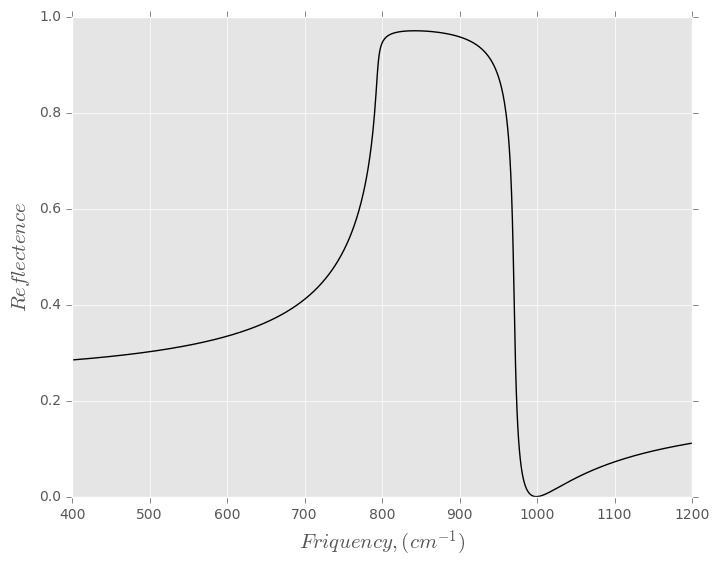
\includegraphics[width=0.9\linewidth]{img/piezo/1.eps}
% {Положение максимума}
% \includegraphics[width=0.9\linewidth]{img/piezo/3.eps}
% {Полуширина}
% \includegraphics[width=0.9\linewidth]{img/piezo/4.eps}
% {Интенсивность в пике}
% \label{ris:500ord}
% \end{figure}
% \vspace{30mm}
% \textcolor{BrickRed}{\subsection{1000 В}}
% Ниже приводится зависимость от времени. Также видно влияние кондиционера на положение пика.
% \begin{figure}[h]
% \centering
% \includegraphics[width=0.9\linewidth]{img/piezo_all/3.eps}
% {Положение максимума}
% 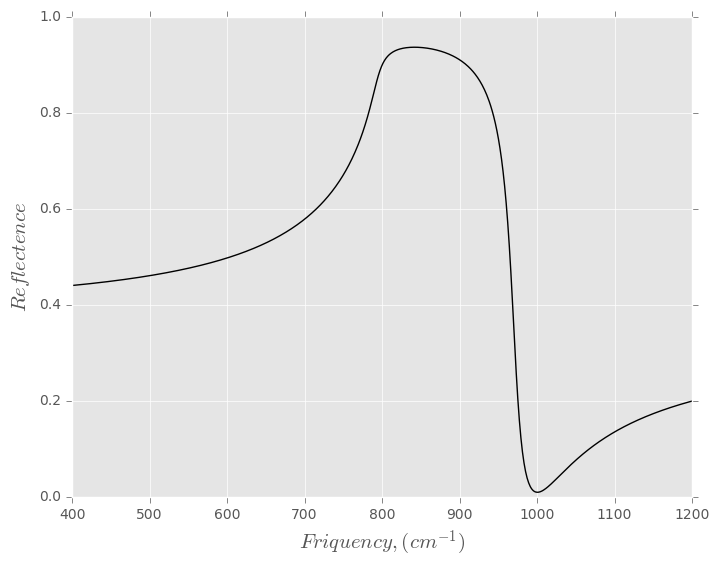
\includegraphics[width=0.9\linewidth]{img/piezo_all/7.eps}
% {Полуширина}
% 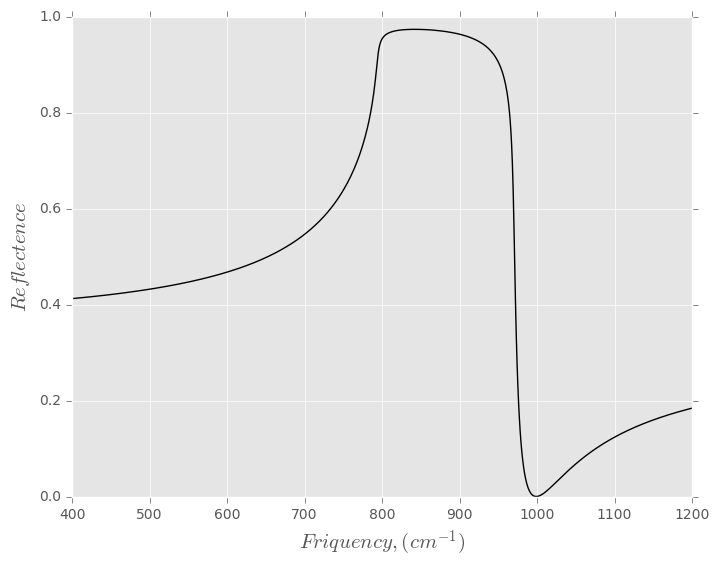
\includegraphics[width=0.9\linewidth]{img/piezo_all/8.eps}
% {Интенсивность в пике}
% \label{ris:1000ord}
% \end{figure}
% \clearpage
% \textcolor{BrickRed}{\subsection{-500 В, -1500В}}
% Ниже приводится зависимость от времени. Также видно влияние кондиционера на положение пика.
% \begin{figure}[h]
% \centering
% 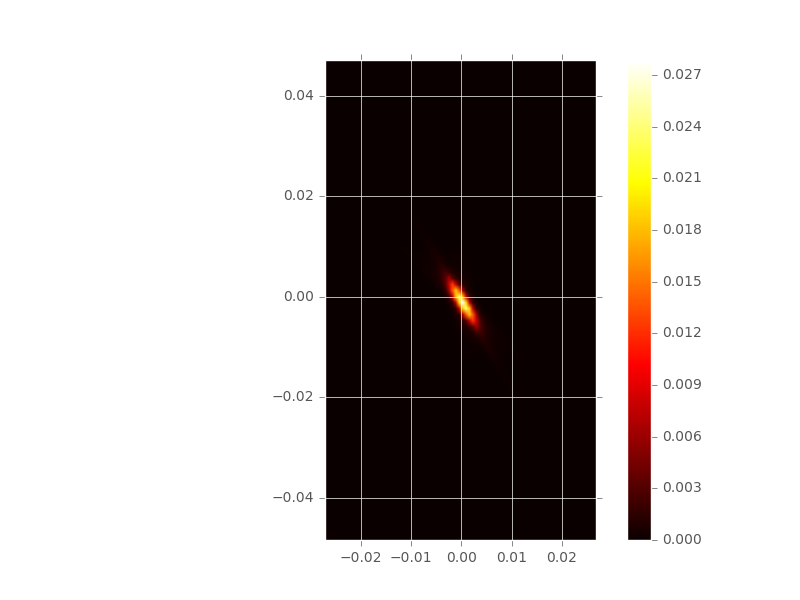
\includegraphics[width=0.85\linewidth]{img/piezo_30/2.eps}
% {Положение максимума}
% \includegraphics[width=0.85\linewidth]{img/piezo_30/3.eps}
% {Полуширина}
% \includegraphics[width=0.85\linewidth]{img/piezo_30/4.eps}
% {Интенсивность в пике}
% \includegraphics[width=0.85\linewidth]{img/piezo_30/5.eps}
%  {Температура}
% \label{ris:-500ord}
% \end{figure}

% \clearpage 
% \section*{Приложение А}
% \begin{itemize}
% 	\item Происходит движение кривой при изменении температуры;
% 	\item Кривая начинается уширяться после 3 сек с момента включения поля
% 	\item Растет пиковая интенсивность
% 	\item Наблюдается зависимость предыдущих измерений, так например если подавать импульс напряжения в одном направлении (-1000) - кривая смещается вправо (например), изменив напряжение на противоположенное (+1000): 1 импульс - КДО движется влево (правильное направление), 2-8 импульс так же происходит смещение в влево, но величина смещения уменьшатся до нуля и мы снова (9-10-.. импульс) наблюдаем смещение вправо.
% 	\item Иногда наблюдается борьба каких-то эффектов, подаем поле резкое движение в одну сменяется на противоположенное(зигзаг)
% 	\item Если подавать ``большое'' напряжение, кривая (форма) может не вернуться с свое первоначальное состояние (останется уширенной, завышенная пиковая интенсивность), времена релаксации в пределах 1 часа.
% 	\item Возможно есть предел на сжатие - 2.6 сек
% \end{itemize}


% \section*{Приложение Б}
% \begin{itemize}
% 	\item Перед каждым измерением вставать в максимум, либо снимать КДО полностью, т.к возникает дополнительная ошибка из - за изменение в пиковой интенсивности от измерения к измерению (время от времени) 
% \end{itemize}

% \section*{Проверить}
% \begin{itemize}
% 	\item Для +1200В - смещение вправо, для +800В - влево
% 	\item Зависимость от температуры

% \end{itemize}

% $^1$ 
% % \begin{figure}[h]
% %\includegraphics[width=0.5\linewidth]{pict/5.png}
% %\end{figure}
 




\end{document}


